\documentclass[../main.tex]{subfiles}
\begin{document}
Un vettore serve per rappresentare oggetti multidimensionali, ad esempio per le informazioni di un aereo potremmo avere un vettore con [velocità, direzione, altezza, potenza] o più semplicemente per descrivere una velocità potremmo usare $\vec{v} = [V_x, V_y]$.

\subsection{Operazioni fondamentali}
\subsubsection{La somma}
Quando sommiamo due vettori quello che facciamo effettivamente è la somma dei componenti, è importante che i due vettori abbiano la stessa dimensione, vale quindi:
$$
    x=[x_1,...,x_n], y=[y_1,...,y_n]\in \mathbb{R}^n \Rightarrow 
    x+y=[x_1+y_1,...,x_n+y_n]
$$

Le modalità di somma dei vettori da un punto di vista geometrico sono principalmente due:
\begin{enumerate}
    \item Metodo del parallelogramma: $AB+AC=AD$
    \begin{center}
        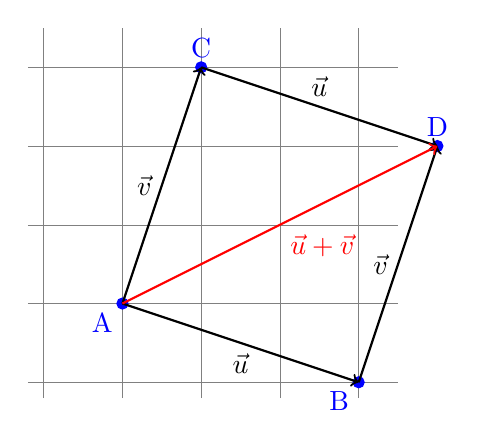
\begin{tikzpicture}
            % Disegna la griglia
            \draw[very thin, gray] (-0.2,-0.2) grid (4.5,4.5);
    
            % Disegna i punti
            \filldraw[blue] (1,1) circle (2pt) node[anchor=north east] {A};
            \filldraw[blue] (4,0) circle (2pt) node[anchor=north east] {B};
            \filldraw[blue] (2,4) circle (2pt) node[anchor=north east, above] {C};
            \filldraw[blue] (5,3) circle (2pt) node[anchor=north east, above] {D};
            
            % Definizione dei vettori
            \draw[->, thick, black] (1,1) -- (4,0) node[midway, below] {$\vec{u}$};
            \draw[->, thick, black] (4,0) -- (5,3) node[midway, left] {$\vec{v}$};
            \draw[->, thick, black] (1,1) -- (2,4) node[midway, left] {$\vec{v}$};
            \draw[->, thick, black] (2,4) -- (5,3) node[midway, above] {$\vec{u}$};
    
            % Somma dei vettori
            \draw[->, thick, red] (1,1) -- (5,3) node[midway, below right] {$\vec{u} + \vec{v}$};
        \end{tikzpicture}
    \end{center}

    \item Metodo punta-coda: $AB+BD=AD$
    \begin{center}
        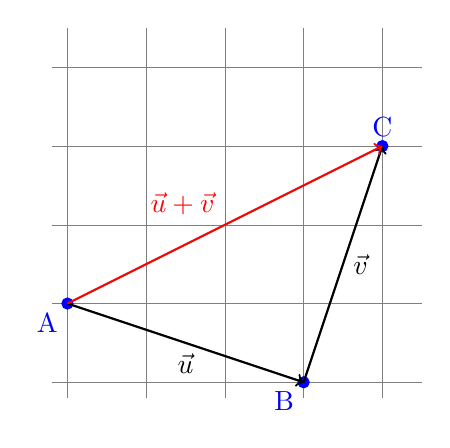
\begin{tikzpicture}
            % Disegna la griglia
            \draw[very thin, gray] (-0.2,-0.2) grid (4.5,4.5);

            % Disegna i punti
            \filldraw[blue] (0,1) circle (2pt) node[anchor=north east] {A};
            \filldraw[blue] (3,0) circle (2pt) node[anchor=north east] {B};
            \filldraw[blue] (4,3) circle (2pt) node[anchor=north east, above] {C};

             % Definizione dei vettori
            \draw[->, thick, black] (0,1) -- (3,0) node[midway, below] {$\vec{u}$};
            \draw[->, thick, black] (3,0) -- (4,3) node[midway, right] {$\vec{v}$};

            % Somma dei vettori
            \draw[->, thick, red] (0,1) -- (4,3) node[midway, above left] {$\vec{u} + \vec{v}$};
        \end{tikzpicture}
    \end{center}
\end{enumerate}


\subsubsection{Moltiplicazione scalare}
È possibile moltiplicare un qualsiasi vettore con un numero reale $k$, il prodotto di tale operazione è un vettore $kx$ che ha al suo interno il valore di ogni suo componente moltiplicato per $k$, ovvero:
$$
    x=[x_1,...,x_n]\in \mathbb{R}^n, k\in \mathbb{R} \Rightarrow 
    kx=[kx_1,kx_2,...,kx_n]
$$

Ecco un semplice esempio di una moltiplicazione di un vettore con un numero reale:
$$
    3 \begin{pmatrix}
        -4 \\
        -3 \\
        \phantom{-}3 \\
        -5 \\
        \phantom{-}3
    \end{pmatrix} =
    \begin{pmatrix}
        3 \cdot (-4) \\
        3 \cdot (-3) \\
        3 \cdot \phantom{(-}3 \phantom{)}\\
        3 \cdot (-5) \\
        3 \cdot \phantom{(-}3 \phantom{)}
    \end{pmatrix} =
    \begin{pmatrix}
        -12 \\
        -9 \\
        \phantom{-}9 \\
        -15 \\
        \phantom{-}9
    \end{pmatrix}
$$    

\subsection{Combinazioni lineari}
Si chiama combinazione lineare dei vettori $x_1,x_2,...,x_m$ con coefficienti (numeri scalari) $c_1,c_2,...,c_m$ il vettore
$$
    c_1x_1+c_2x_2+...+c_mx_m
$$
Il risultato di questa somma apparterrà allo spazio vettoriale di partenza.
\vspace{1cm}

Facciamo un semplice esempio per rendere meglio l'idea, mettiamo caso che dati due vettori $u=[5, -8, -5]$ e $v=[-6, 5, -6]$, vogliamo trovare la combinazione lineare $2u-3v$:
$$
    2 \begin{pmatrix}
        \phantom{-}5 \\
        -8 \\
        -5
    \end{pmatrix} -3
    \begin{pmatrix}
        -6 \\
        \phantom{-}5 \\
        -6
    \end{pmatrix} = 
    \begin{pmatrix}
        \phantom{-}28 \\
        -31 \\
        \phantom{-}8
    \end{pmatrix}
$$

Ora da un punto di vista geometrico cerchiamo di esprimere $AE$ e $AF$ come combinazioni lineari dei due vettori $\vec{a}=AB$ e $\vec{b}=AC$.
\begin{center}
    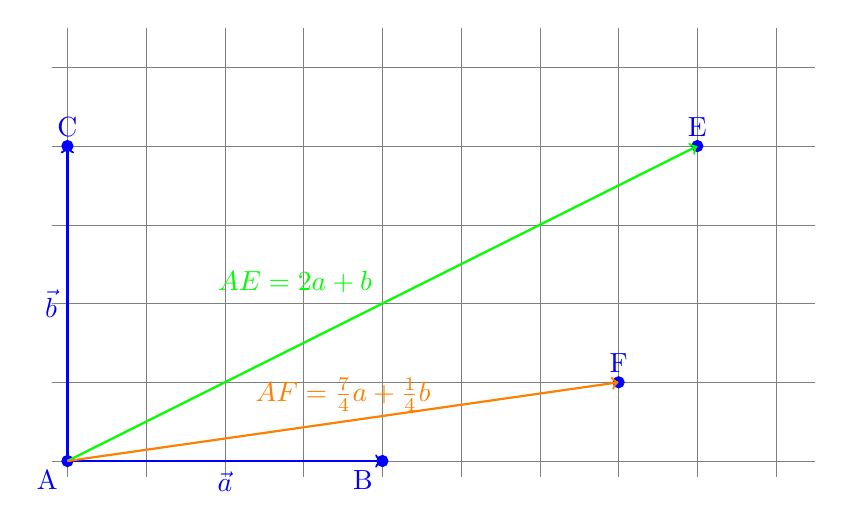
\begin{tikzpicture}
        % Disegna la griglia
        \draw[very thin, gray] (-0.2,-0.2) grid (9.5,5.5);

         % Disegna i punti
        \filldraw[blue] (0,0) circle (2pt) node[anchor=north east] {A};
        \filldraw[blue] (4,0) circle (2pt) node[anchor=north east] {B};
        \filldraw[blue] (0,4) circle (2pt) node[anchor=north east, above] {C};
        \filldraw[blue] (8,4) circle (2pt) node[anchor=north east, above] {E};
        \filldraw[blue] (7,1) circle (2pt) node[anchor=north east, above] {F};

         % Definizione dei vettori
        \draw[->, thick, blue] (0,0) -- (4,0) node[midway, below] {$\vec{a}$};
        \draw[->, thick, blue] (0,0) -- (0,4) node[midway, left] {$\vec{b}$};

        % Somma dei vettori
        \draw[->, thick, green] (0,0) -- (8,4) node[midway, above left] {$AE=2a+b$};
        \draw[->, thick, orange] (0,0) -- (7,1) node[midway, above] {$AF=\frac{7}{4}a+\frac{1}{4}b$};
    \end{tikzpicture}
\end{center}

%\textbf{Nota:} se due vettori sono paralleli (cioè hanno la stessa direzione) la loro somma sarà anch'essa parallela ai vettori originali. Possiamo quindi determinare
%se due vettori sono paralleli ($x \parallel y$ ) stabilendo se esiste un numero reale $k$ tale che $y=kx$. 0 è parallelo a qualunque vettore.
%Se al contrario due vettori non sono paralleli, la loro somma darà come risultato un vettore con una direzione diversa rispetto ad entrambi.
\vspace{1.5cm}
\subsubsection{Generare tutti i vettori di $\mathbb{R}^2$}
\textbf{Teorema:} se $\vec{u},\vec{v} \in \mathbb{R}^2$ sono non paralleli, allora è possibile esprimere qualunque vettore $\vec{w}$ di $\mathbb{R}^2$ come combinazione lineare di $\vec{u}$ e $\vec{v}$ in un \underline{unico} modo.

Per rappresentare un vettore come combinazione lineare di altri due vettori occorre creare un sistema e separare le componenti.
\textbf{Esempio:} esprimere $\vec{w}= \lbrack6,4\rbrack$ come CL dei vettori $\vec{u}=\lbrack3,1\rbrack$ e $\vec{v}=\lbrack1,2\rbrack$
$$
    \begin{pmatrix}
        6 \\
        4
    \end{pmatrix}
    = h \begin{pmatrix}
        3 \\
        1
    \end{pmatrix}
    +k \begin{pmatrix}
        1 \\
        2
    \end{pmatrix} \rightarrow
    \begin{cases}
        6 = 3h+k \\
        4 = h+2k
    \end{cases}
$$
Un sistema del genere avrà una soluzione solo se $\vec{u}$ e $\vec{v}$ non sono paralleli, in caso contrario ($\vec{u} || \vec{v}$) il risultato del sistema risulterà impossibile.
In questo caso, sviluppando il sistema troviamo che $h = \frac{8}{5}, k=\frac{6}{5}$.
\pagebreak

\textbf{Esempio:} esiste una combinazione lineare dei vettori $\vec{u}= \lbrack6,4\rbrack$ e $\vec{v}= \lbrack9,6\rbrack$ che dia il vettore $\vec{w}= \lbrack12,10\rbrack$?
$$
    h \begin{pmatrix}
        6 \\
        4
    \end{pmatrix}
    +k \begin{pmatrix}
        9 \\
        6
    \end{pmatrix}
    = \begin{pmatrix}
       12 \\
       10
    \end{pmatrix} \rightarrow
    \begin{cases}
        6h+9k=12 \\
        4h+6k=10
    \end{cases}
$$

Provando a risolvere il sistema si ottiene $8=10$ (il sistema non ammette soluzioni), quindi non è possibile esprimere
$\vec{w}= \lbrack12,10\rbrack$ come combinazione lineare dei vettori $\vec{u}= \lbrack6,4\rbrack$ e $\vec{v}= \lbrack9,6\rbrack$,
ciò significa che $\vec{u}$ e $\vec{v}$ \textbf{sono paralleli}. In altre parole combinando linearmente questi due vettori si possono ottenere \textbf{solo} i vettori che hanno la stessa direzione di $\vec{u}$ e $\vec{v}$. Graficamente risulta così:
\begin{figure}[h]
    \centering
    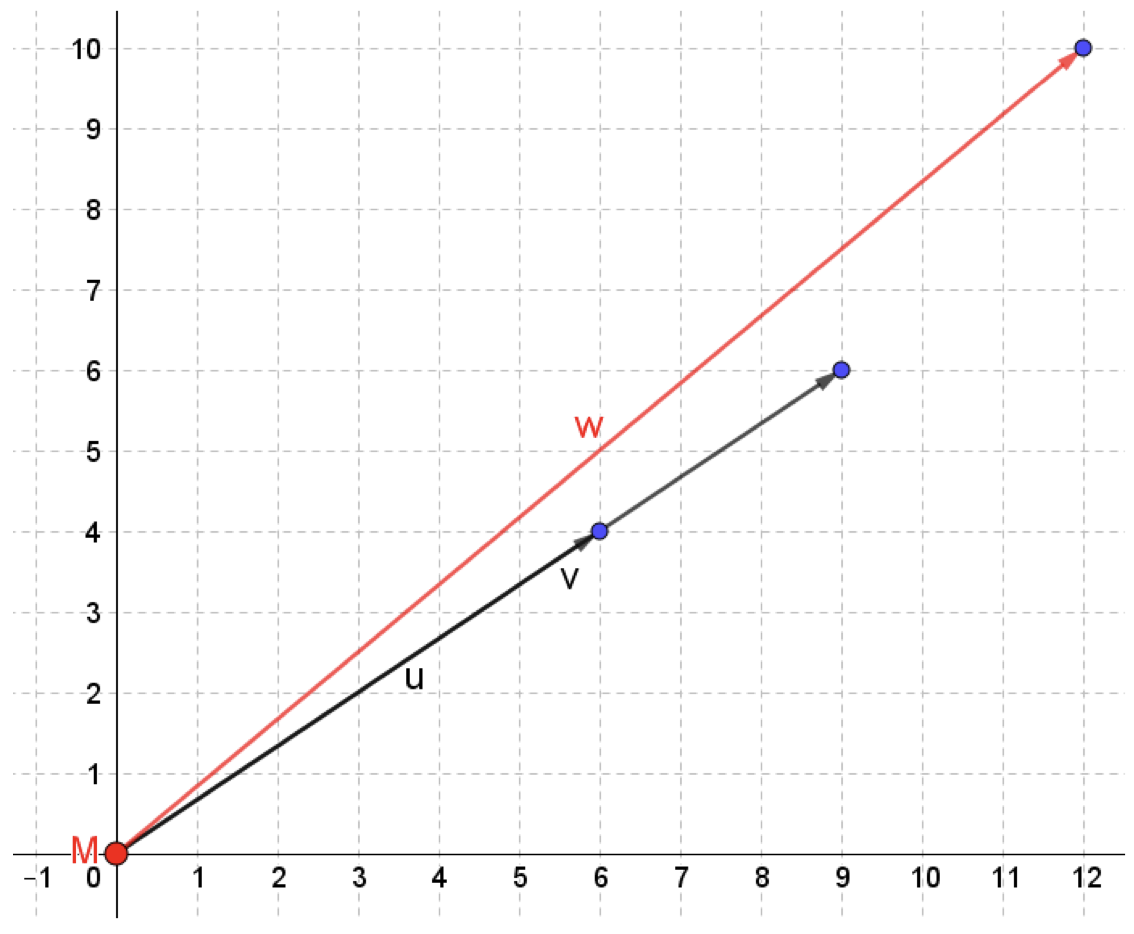
\includegraphics[width=0.6\textwidth]{../images/vettoriParalleli.png}
\end{figure}

\subsubsection{Generare tutti i vettori di $\mathbb{R}^3$}
\textbf{Teorema:} se $\vec{u},\vec{v},\vec{w} \in \mathbb{R}^3$ sono non complanari (non appartengono allo stesso piano e quindi nessuno di essi si può  esprimere come combinazione lineare degli altri due), allora è possibile esprimere qualunque vettore $\vec{z}$ di $\mathbb{R}^3$ come combinazione lineare di $\vec{u},\vec{v},\vec{w}$ in un \underline{unico} modo.

In questo caso, utilizzando \textbf{due} vettori non paralleli, possiamo generare un piano su $\mathbb{R}^3$, tuttavia in questo caso
avendo una dimensione 3 e soltanto due vettori, siamo limitati a generare \textbf{solo} i vettori che si trovano sul piano dei due vettori.
\begin{figure}[h]
    \centering
    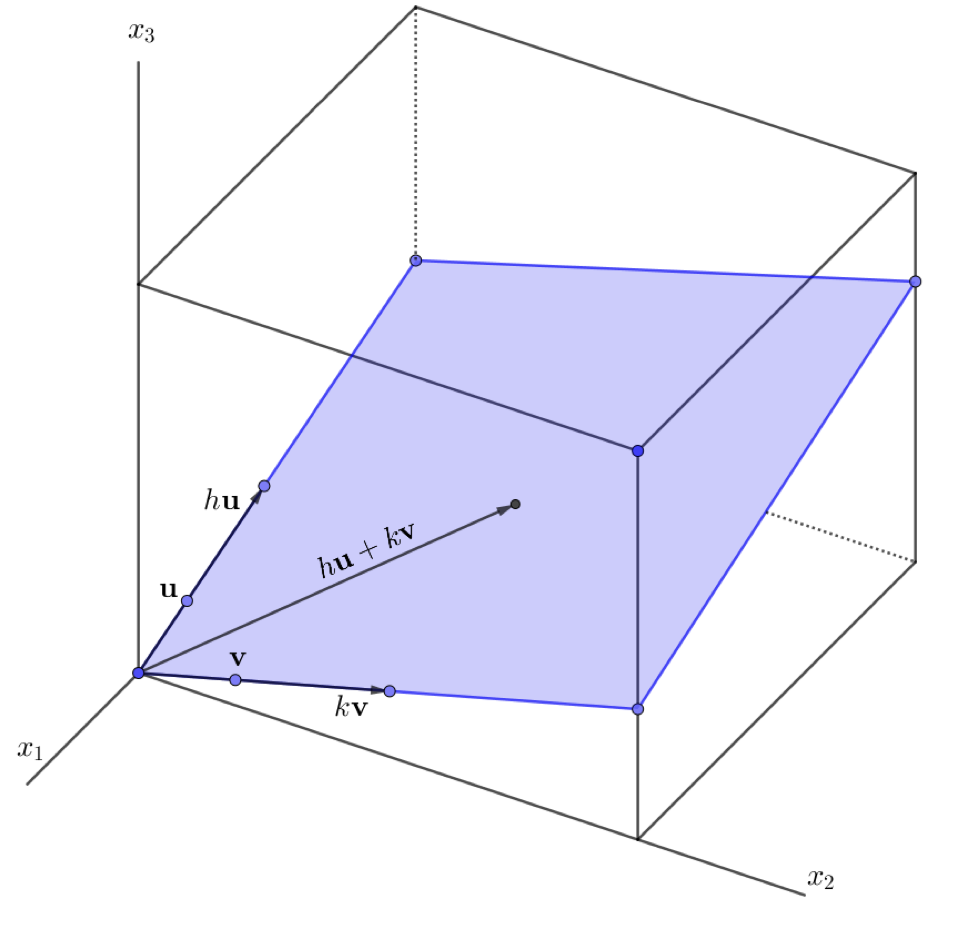
\includegraphics[width=0.3\textwidth]{../images/combinazioneLineareR3.png}
\end{figure}

Per generare tutti i vettori possibili occorrono quindi 3 vettori, possono essere vettori qualsiasi purché non siano complanari, ovvero nessuno di essi si possa esprimere come combinazione lineare degli altri.

%Avendo tre vettori $\vec{w}$, $\vec{u}$ e $\vec{v}$, se $\vec{w}$ non si può esprimere come combinazione lineare degli altri due significa che abbiamo tre vettori validi per poter generare ogni vettore in $\mathbb{R}^3$.

In generale, per generare i vettori di $\mathbb{R}^n$ sono necessari e sufficienti $n$ vettori, purché nessuno di essi si possa esprimere come combinazione lineare degli altri.

\subsubsection{CAS Geogebra}
Abbiamo capito quindi che per determinare una combinazione lineare tra più vettori è importante riuscire a creare un sistema di equazioni. Per quanto riguarda però la risoluzione possiamo usare il CAS di Geogebra, tramite lo strumento Risolvi gli passiamo come parametri la lista di equazioni e le variabili di riferimento.
\begin{figure}[h]
    \centering
    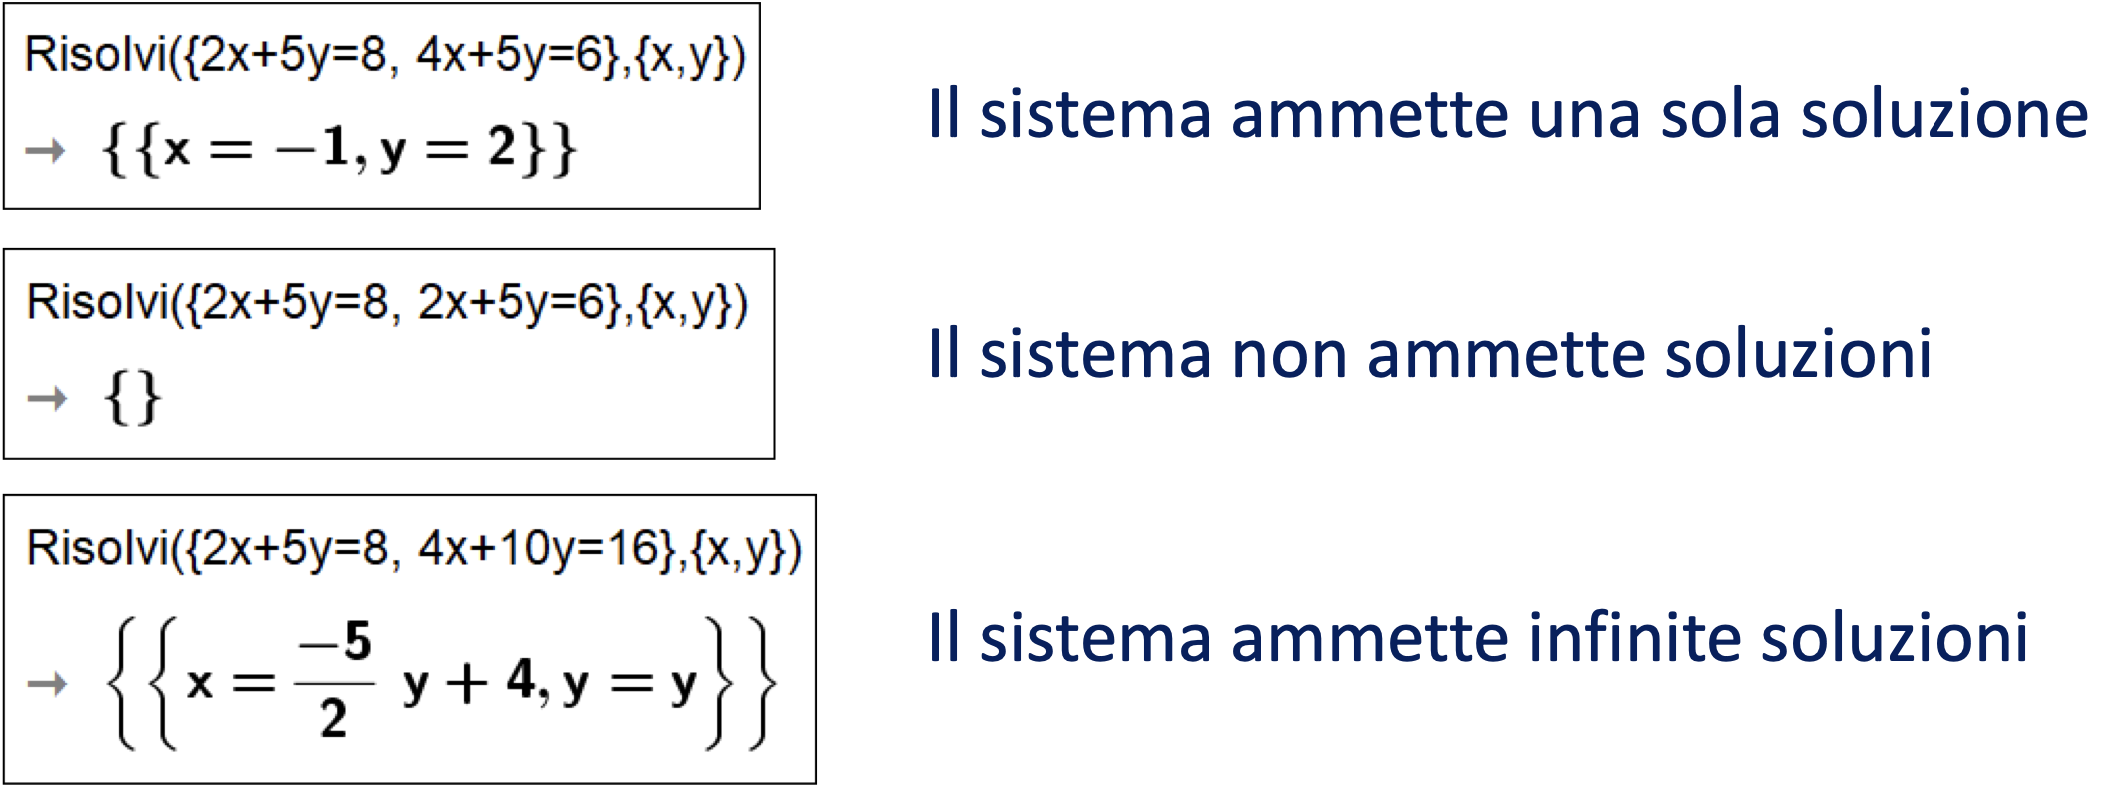
\includegraphics[width=1\textwidth]{../images/casGeogebra.png}
\end{figure}
\pagebreak

\subsection{Dipendenza e indipendenza lineare}
Si dice che i vettori $x_1,...,x_m \in \mathbb{R}^n$ sono \textbf{linearmente indipendenti (LI)} se nessuno di essi si può esprimere come combinazione lineare degli altri,
altrimenti si dicono \textbf{linearmente dipendenti (LD)}.

Possiamo dire quindi che una \textbf{base} di $\mathbb{R}^n$ è formata da $n$ vettori \textbf{linealmente indipendenti}.
Una \textbf{base} è una lista di vettori LI che generano $\mathbb{R}^n$.
\vspace{1cm}

\textbf{Teorema}. I vettori $x_1...x_m \in \mathbb{R}^n$ sono \textbf{linearmente indipendenti} se e solo se l'unica loro combinazione lineare
che dà il vettore nullo $0$ è la combinazione banale:
$$
    0x_1 + ... + 0x_m = 0
$$
In questo modo occorre risolvere un solo sistema lineare \textbf{omogeneo} (con i termini noti tutti nulli).

Se ad esempio vogliamo stabilire se i vettori $a \begin{pmatrix}1 \\ 2 \\ 3 \end{pmatrix}, b \begin{pmatrix}4 \\ 5 \\ 6 \end{pmatrix}, c \begin{pmatrix}7 \\ 8 \\ 9 \end{pmatrix}$
sono LI o LD, diventa:
$$
    h \begin{pmatrix}
        1 \\
        2 \\
        3
    \end{pmatrix}
    +j \begin{pmatrix}
        4 \\
        5 \\
        6
    \end{pmatrix}
    +k \begin{pmatrix}
        7 \\
        8 \\
        9
    \end{pmatrix}
    = \begin{pmatrix}
       0 \\
       0 \\
       0
    \end{pmatrix}
$$

\vspace{1cm}
\subsubsection{Interpretare i risultati}
Una volta che abbiamo il sistema, possiamo inserirlo in Geogebra utilizzando la funzione \textbf{Risolvi} con la sintassi vista nel capitolo
scorso. Se l'unico valore possibile dei coefficienti è $0$ (ammette \textbf{solo} la soluzione banale), allora i vettori sono LI.
\begin{figure}[h]
    \centering
    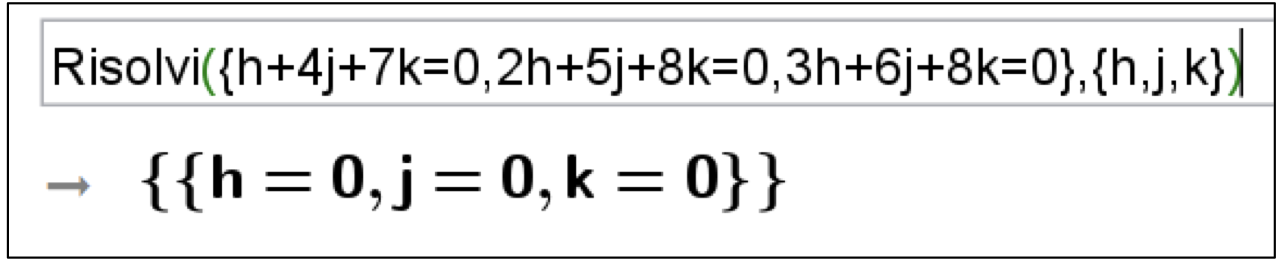
\includegraphics[width=0.4\textwidth]{../images/casLI.png}
\end{figure}

In caso contrario, significa che i vettori sono LD.
\begin{figure}[h]
    \centering
    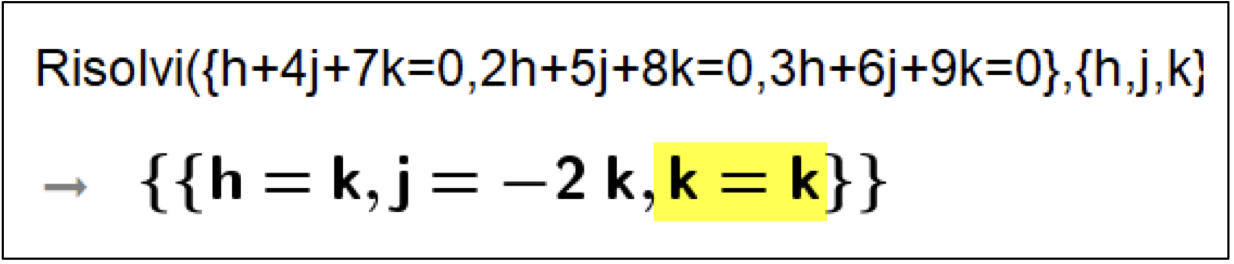
\includegraphics[width=0.4\textwidth]{../images/casLD.png}
\end{figure}

\vspace{1cm}
Facciamo un esempio più pratico per notare qualche altro dettaglio. Proviamo a stabilire se i vettori $a \begin{pmatrix}1 \\ 2 \\ 3 \\ 4 \end{pmatrix}, b \begin{pmatrix}5 \\ 6 \\ 7 \\ 8\end{pmatrix}, c \begin{pmatrix}9 \\ 10 \\ 11 \\ 12 \end{pmatrix}, d \begin{pmatrix}13 \\ 14 \\ 15 \\ 16 \end{pmatrix}$
sono LI o LD.

\begin{figure}[h]
    \centering
    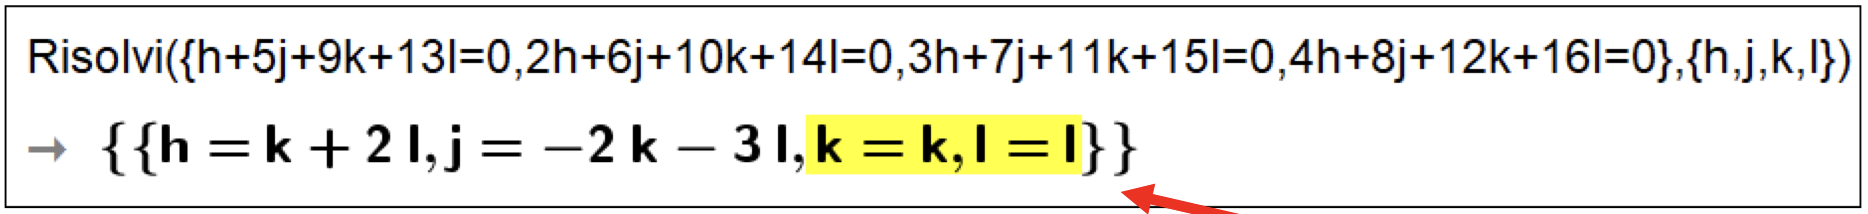
\includegraphics[width=0.7\textwidth]{../images/casLD2.png}
\end{figure}
Notiamo per prima cosa che i vettori sono LD. Inoltre ci sono due variabili libere ($k=k, l=l$), ciò significa che ci sono solo
2 vettori LI ($4-2 = 2$), per verificare quali dovremmo vedere i singoli casi. Infine sappiamo che $a,b,c,d$ generano un \textbf{sottospazio}
di $\mathbb{R}^4$ di \textbf{dimensione} $2$.

In generale, $k$ vettori LI non nulli di $\mathbb{R}^n$ generano un \textbf{sottospazio} di \textbf{dimensione} $k$.

\end{document}